\documentclass[a4paper, 14pt]{article}
\usepackage{comment}

\usepackage{setspace}
\usepackage{indentfirst}
%% Language and font encodings
\usepackage{extsizes}
\usepackage[english, russian, ukrainian]{babel}
\usepackage[utf8x]{inputenc}
\usepackage[T1]{fontenc}
\linespread{1.6}
%% Sets page size and margins
\usepackage[a4paper,top=2cm,bottom=2cm,left=3cm,right=2cm,marginparwidth=1.75cm]{geometry}

%\usepackage{fontspec}

%% Useful packages
\usepackage{authblk}
\usepackage{amsmath}
\usepackage{graphicx}
\usepackage[colorinlistoftodos]{todonotes}
\usepackage[colorlinks=true, allcolors=black]{hyperref}
\usepackage{tikz}
%\usepackage{subfigure}
\usepackage[lofdepth,lotdepth]{subfig}
\usepackage{float}
\usepackage{multirow}
\usepackage{hhline}
\usepackage{lineno}

%\linenumbers
\renewcommand{\thefigure}{\thesection.\arabic{figure}}

\numberwithin{equation}{section}
\numberwithin{table}{section}

\title{}


\author[1]{V. Haponov}
\author[2]{R. Yermolenko}
\affil[1]{Taras Shevchenko National University of Kiev, Kiev, Ukraine}
\affil[2]{}

\setcounter{Maxaffil}{0}
\renewcommand\Affilfont{\itshape\normalsize}
\renewcommand{\arraystretch}{1.5} %% increase table row spacing
%\renewcommand{\tabcolsep}{1cm}

\date{}
\begin{document}
	
%content

\selectlanguage{ukrainian}
\newpage
\tableofcontents
\newpage
\pagestyle{plain}
\setcounter{page}{2}
	
%end 

\newpage
\section{Глава 1}
\setcounter{figure}{0} 
\subsection{Geant4 MultiThreading}

\subsection{$QGSP\_BERT$}
	$QGSP\_BERT$ - ця фізична модель входить в перелік стандартних фізичних моделей розрахункового пакету Geant4
	Базується на каскадній моделі Бертіні та враховує реакції для нейтронів менше ніж 20 МеВ. Для валідації данної моделі необхідне виконання наступних умов $\frac{\lambda_B}{\nu} \ll \tau_c \ll \Delta{t}$, $\lambda_B$ - хвиля де-Бролля для налітаючої частинки, $\nu$ - швидкість налітаючої частинки, $\Delta{t}$ - час між зіткненнями. Та модель яка лягла в основу коду Geant4 була протестована на частинках з енергіями від 100 МеВ до 3 ГеВ
\subsection{Джерела нейтронів}

\newpage
\section{Глава 2}
\setcounter{figure}{0}
\subsection{Опис детектора}
	
	Для моделювання чутливого об'єму був обраний надчистий германій, з діаметром 60.6 міліметрів, та довжиною 56.7 міліметрів. Рис. ~\ref{ris:s_detector_volume} \\
	
	\begin{figure}[hbt!]
		%\vspace{-10pt}
		\centering 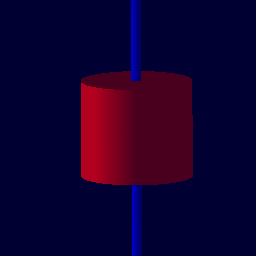
\includegraphics[width=0.7\textwidth]{images/sDetector158cm3.png}
		\caption{Форма чутливого об'єму} 
		\label{ris:s_detector_volume}	
	\end{figure} 

	Детектор буде розміщенний поряд з джерелом нейтронів високих енергій, 14.5 МеВ. Тому детектор був розміщений у трьох шаровий захист. Рис. ~\ref{ris:s_detector_P}
	
	\begin{figure}[hbt!]
		%\vspace{-10pt}
		\centering 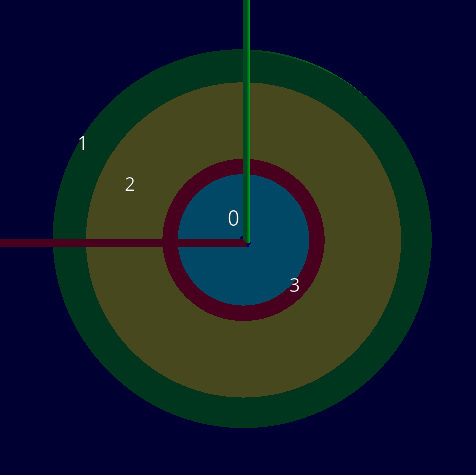
\includegraphics[width=0.7\textwidth]{images/dectorPrt.png}
		\caption{Захист детектора, Al - зелений товщина 2 см., B - жовтий товщина 5 см., Pb - червоний товщина 1 см. Блакитний шар повітря} 
		\label{ris:s_detector_P}	
	\end{figure} 

	В захисті використовується Бор для поглинання теплових нейтронів, так як вся детекторна система буде знаходитися під водою, то нейтрони від джерела будуть втрачати енергію при пружному розсіянні на водню. 
	
	Опис реакцій на захисті -- та сповільнювачі \\
	Опис вторинного альфа випроміннення від Бор --
	Fano factor Ge = 0.13 
	Для утворення пари 3.62 еВ = 300 К

\subsection{Опис джерела}
	
	
\subsection{Опис коду моделі}

	\begin{figure}[hbt!]
		%\vspace{-10pt}
		\centering 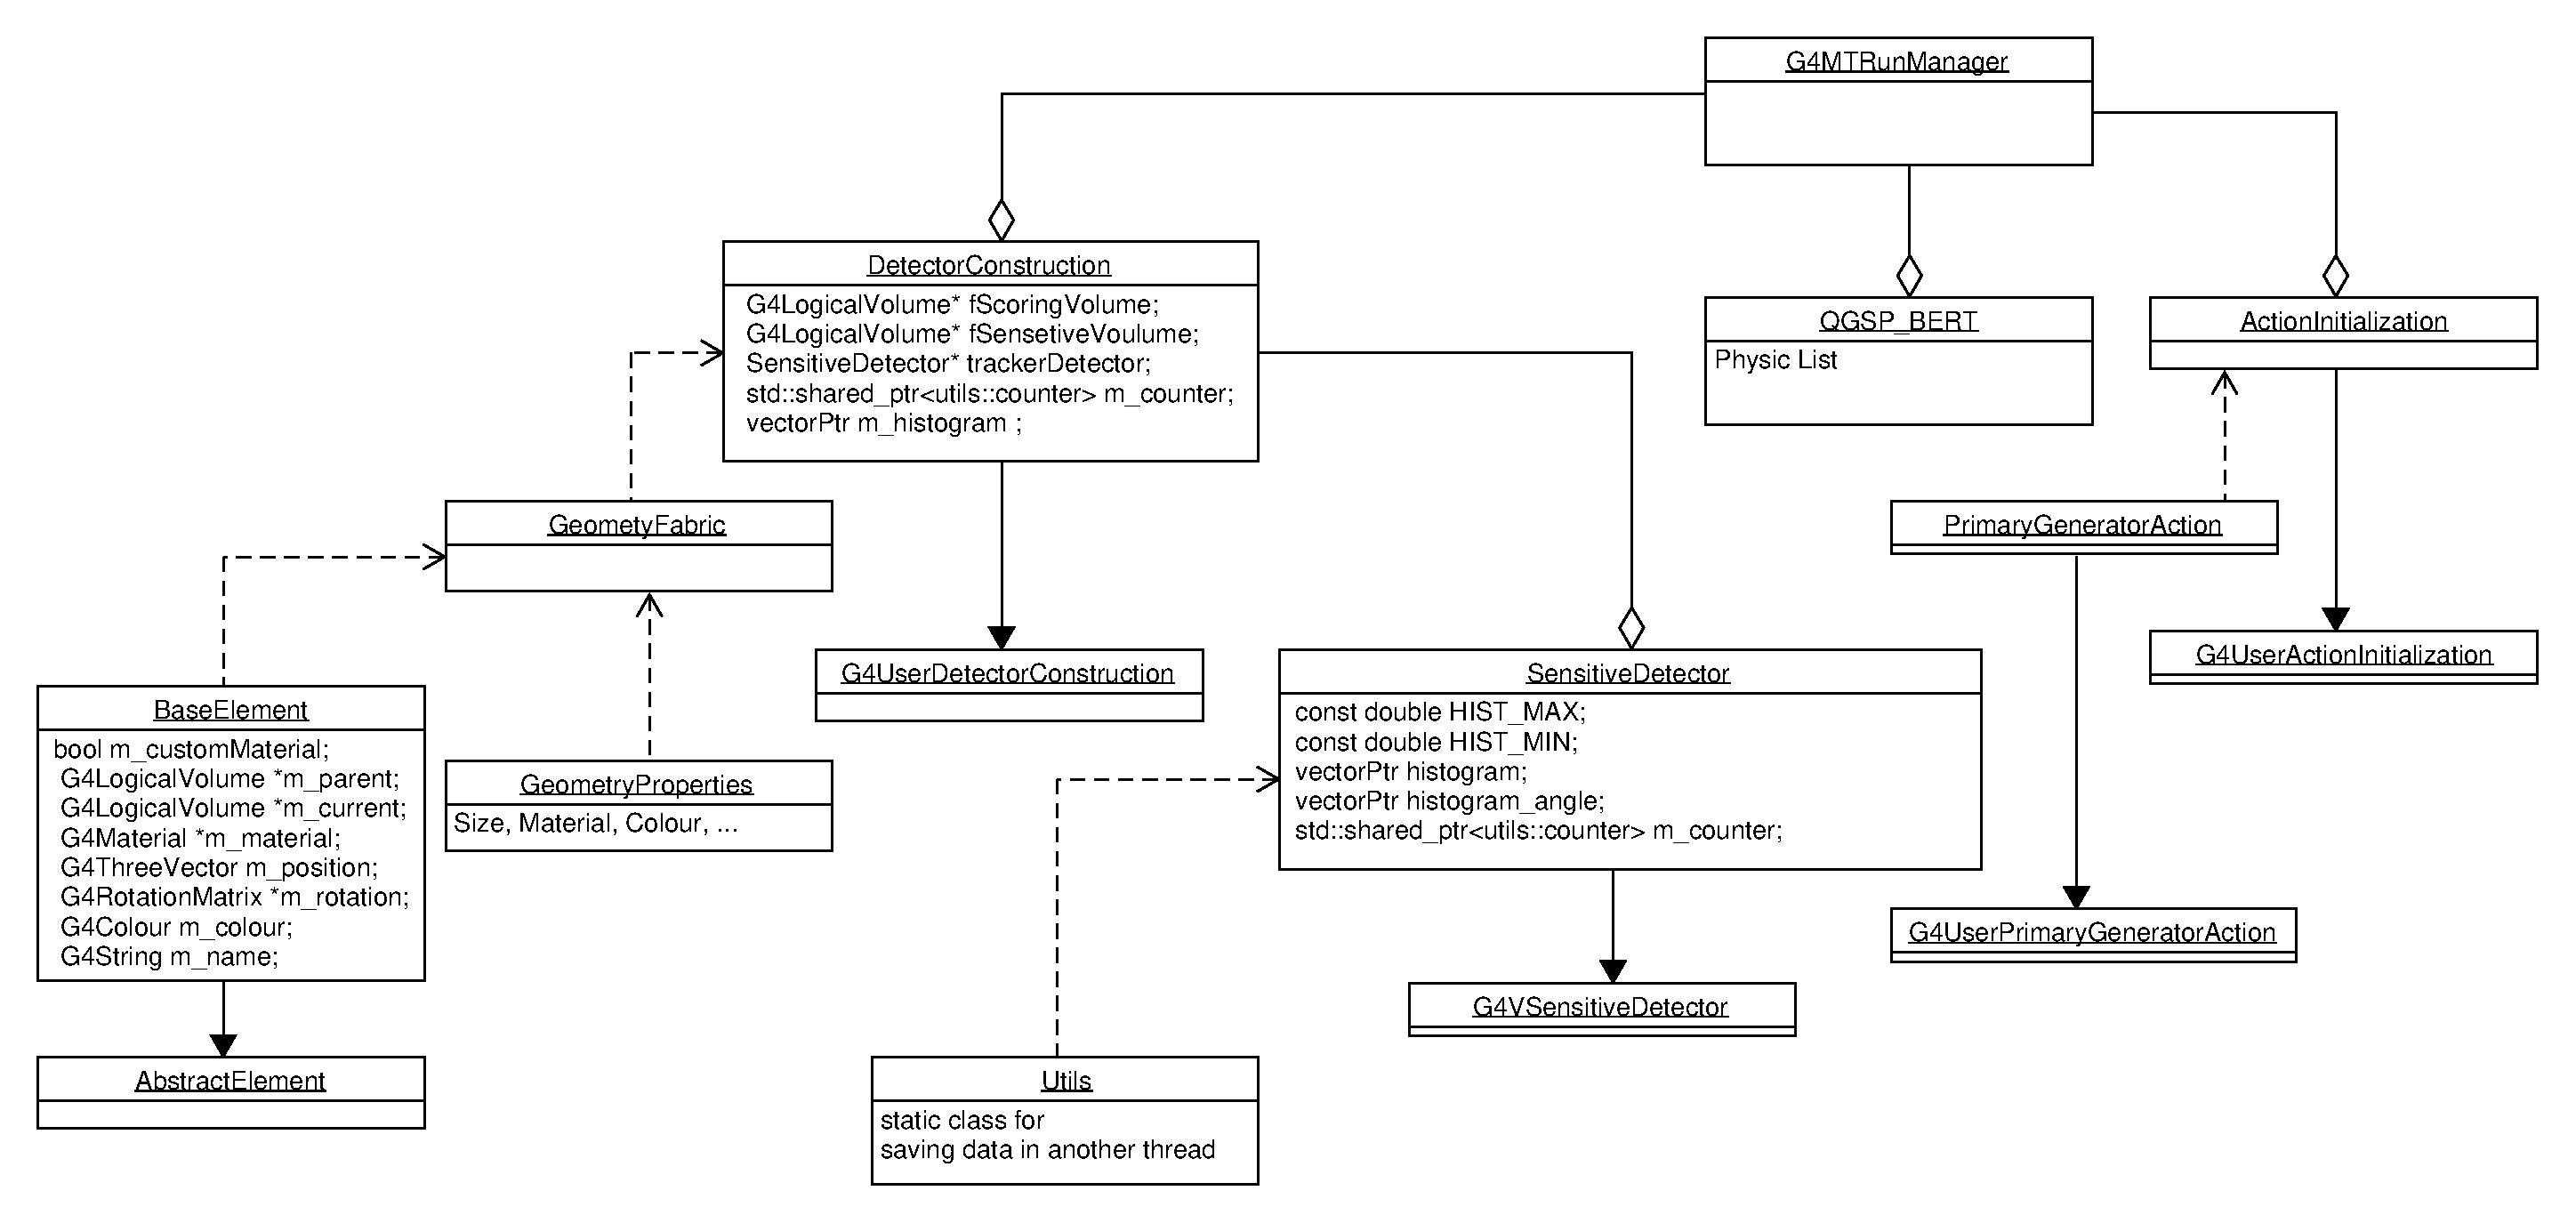
\includegraphics[width=1\textwidth]{res/classDiagram.pdf}
		\caption{Діаграма класів коду моделі} 
		\label{ris:s_classDiagram}	
	\end{figure} 

	Цілью було написати максимально зручний код для набору спектрів за різних умов та на різних мішеннях, тому були створені абстрактні класси для створення геометричних об'єктів. Для зручності створення матеріалів були створенні структури. 
	Та для пришвидшення роботи були всі можливі константи ініціалізувалися на етапі компіляції. Для полегшення контролю над пам'яттю використовувалися розумні вказівники С++ 11 стандарту.
	
\newpage 
\section{Глава 3}
\setcounter{figure}{0}
\subsection{Опис обробки спектру}

В результаті моделювання, чутливим об'ємом набирались апаратні спектри, для чутливого об'єму було встановленно 16384 біни. Далі для наближення спектру до реального, була проведенне його сглажування за наступної формулою $\Delta{E} = 2.36 \sqrt{F  \frac{w}{E}}  w$, $\Delta{E}$ - енергія на один бін, F - Фано фактор, w - кількість енргії на утворення пари, та пронормований на кількість нейтронів з джерела. Так як для спрощення побудови джерела в моделі, використовувалась спрощенна геометрія, а генерація нейтронів відбувалась майже строго у заданому напрямку. Так як джерело нейтронів вважалося ізотропним, то загальна кількіть частинок розраховувалась наступною формолую $ 4 \pi n = N$, де $N -$ це загальна кількість чатсинок.

\subsection{Валідація моделі}

	Для підтвердження можливості проведення наборів на моїй моделі був набраний спектор для Гірчичного газу. Рис ~\ref{ris:MustBackAllLogSm}. Та порівняний з отриманим спектром в статьї <link to source ?help> 	
	\begin{figure}[h!]
		%\vspace{-10pt}
		\centering 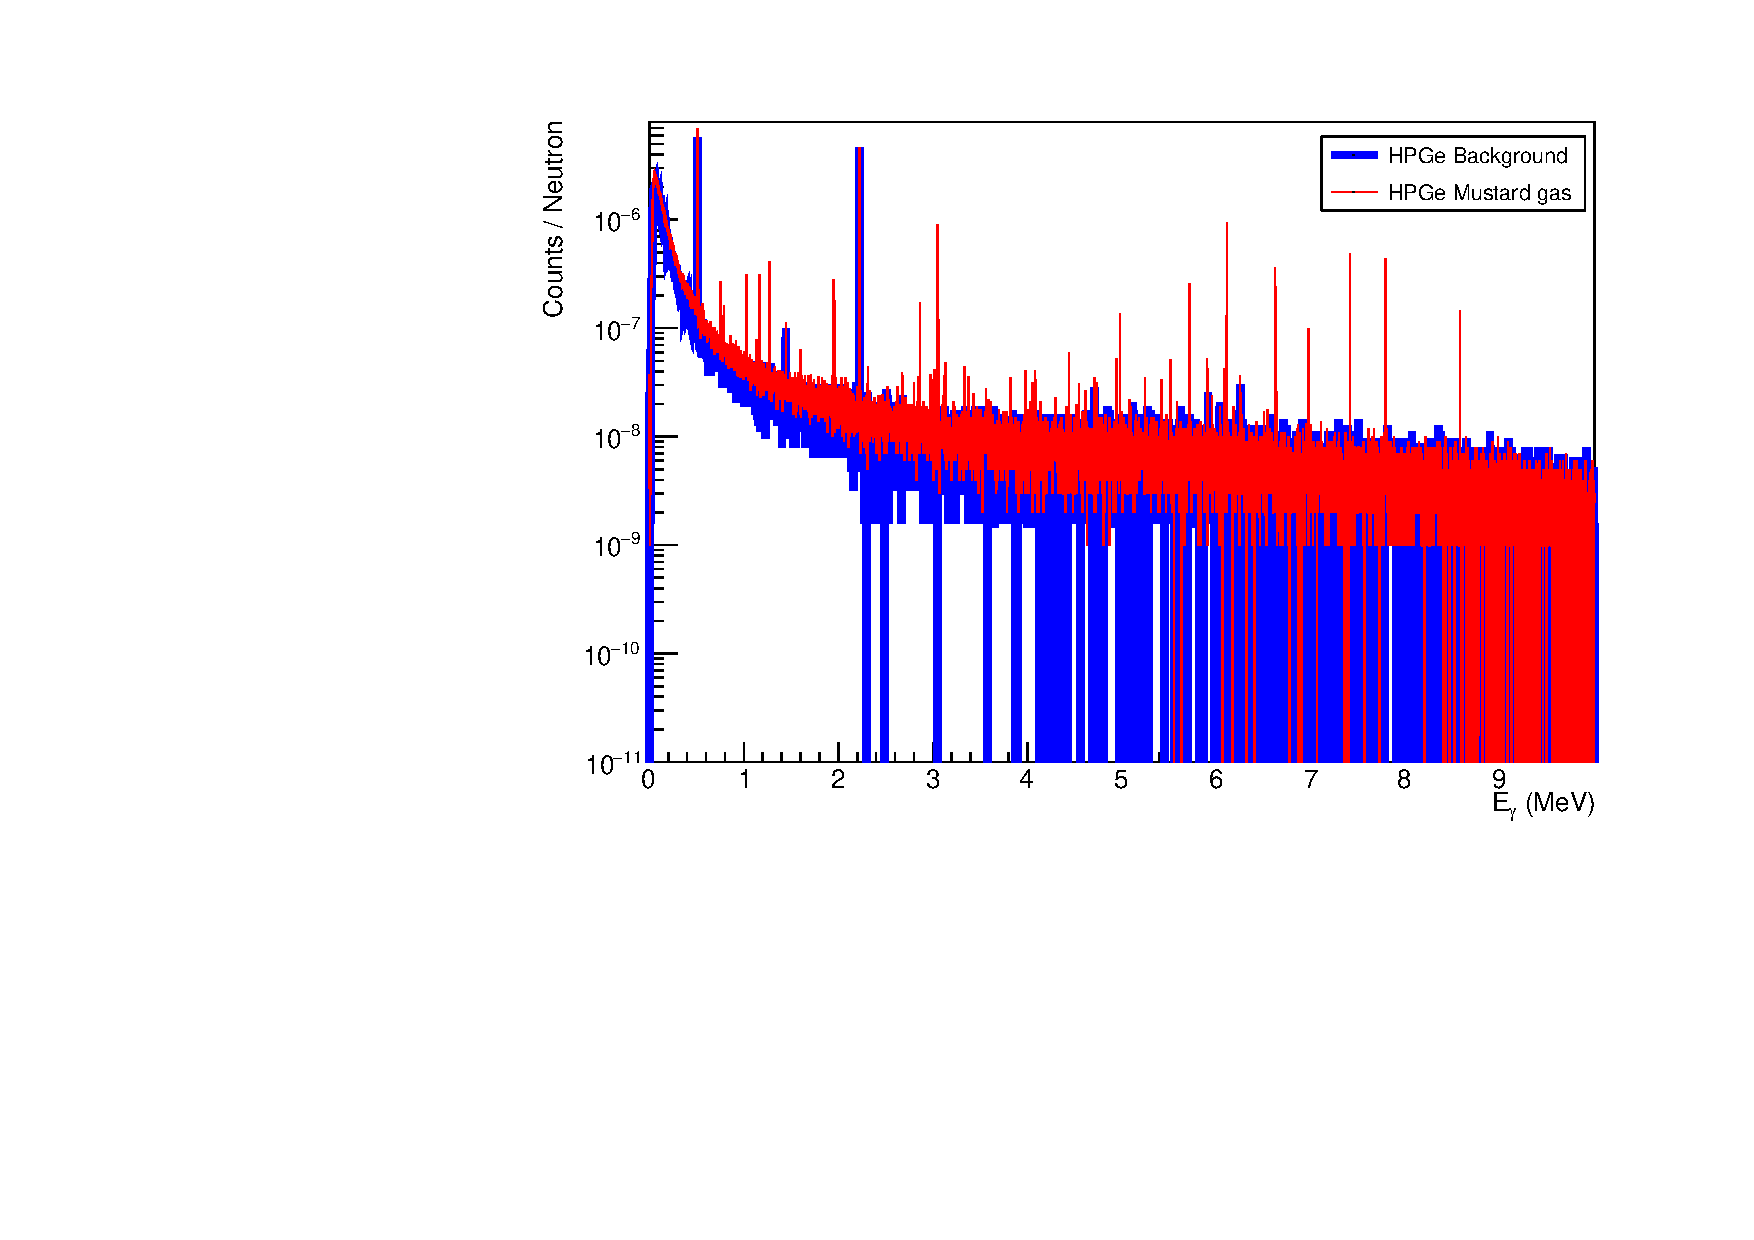
\includegraphics[width=1\textwidth]{res/smMustFonAll.pdf}
		\caption{Червоним - представлений спектор для Гірчичного газу. Синім - фону} 
		\label{ris:MustBackAllLogSm}	
	\end{figure} 
	У висновках до проведеної роботи в данної статьї було вказано, що най більш вираженими і читкіми були лінії Cl 7,42 7,80 8,58 МеВ, також було вказано ряд ліній які їм не вдалося валідувати (перефразувати "лінії") 
	На Рис. ~\ref{ris:MustFon78} - зоображені піки 7.42 та 7.80 МеВ
	Рис.  ~\ref{ris:MustFon89} - 8.58 МеВ	
	\begin{figure}[hbt!]
		%\vspace{-10pt}
		\centering 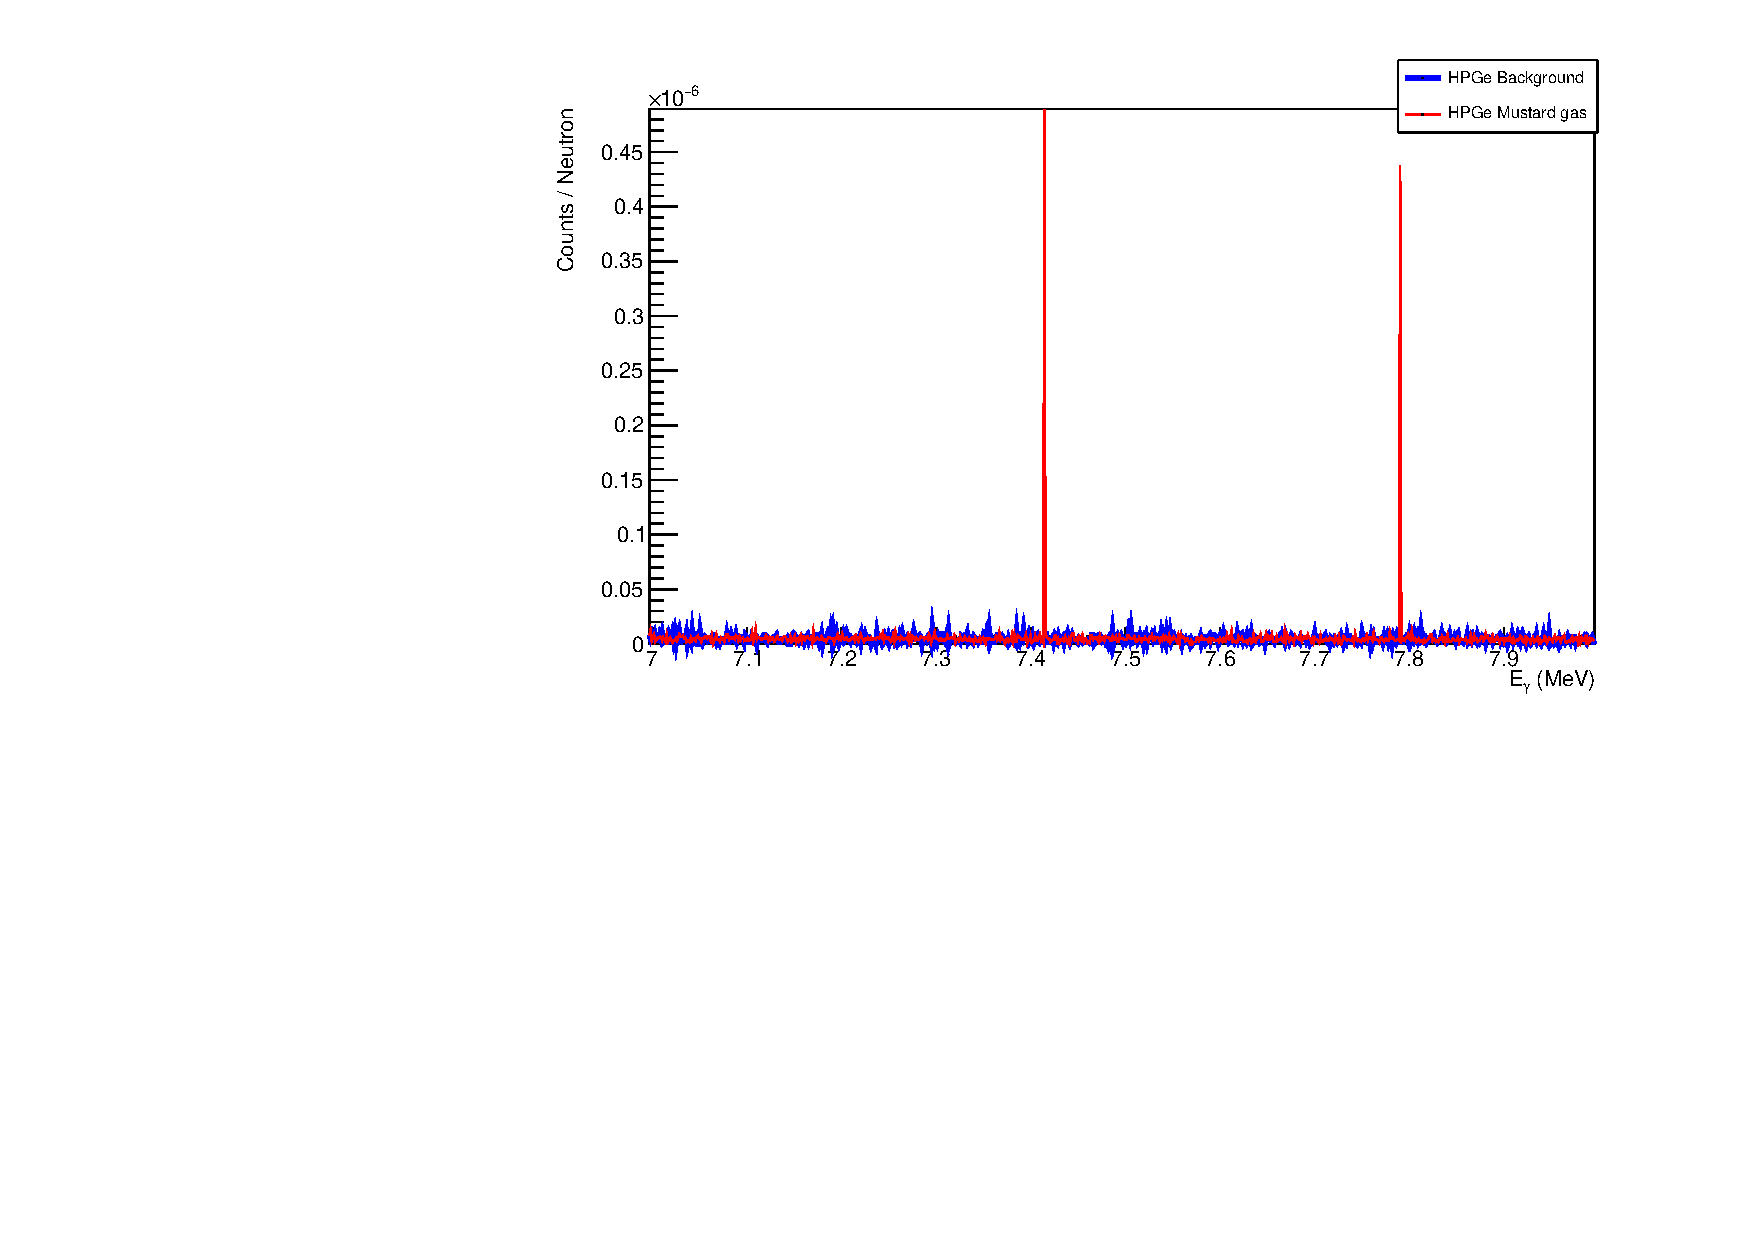
\includegraphics[width=1\textwidth]{res/mustFon78.pdf}
		\caption{Червоним - представлений спектор для Гірчичного газу. Синім - фону} 
		\label{ris:MustFon78}	
	\end{figure} 	
	\begin{figure}[hbt!]
		%\vspace{-10pt}
		\centering 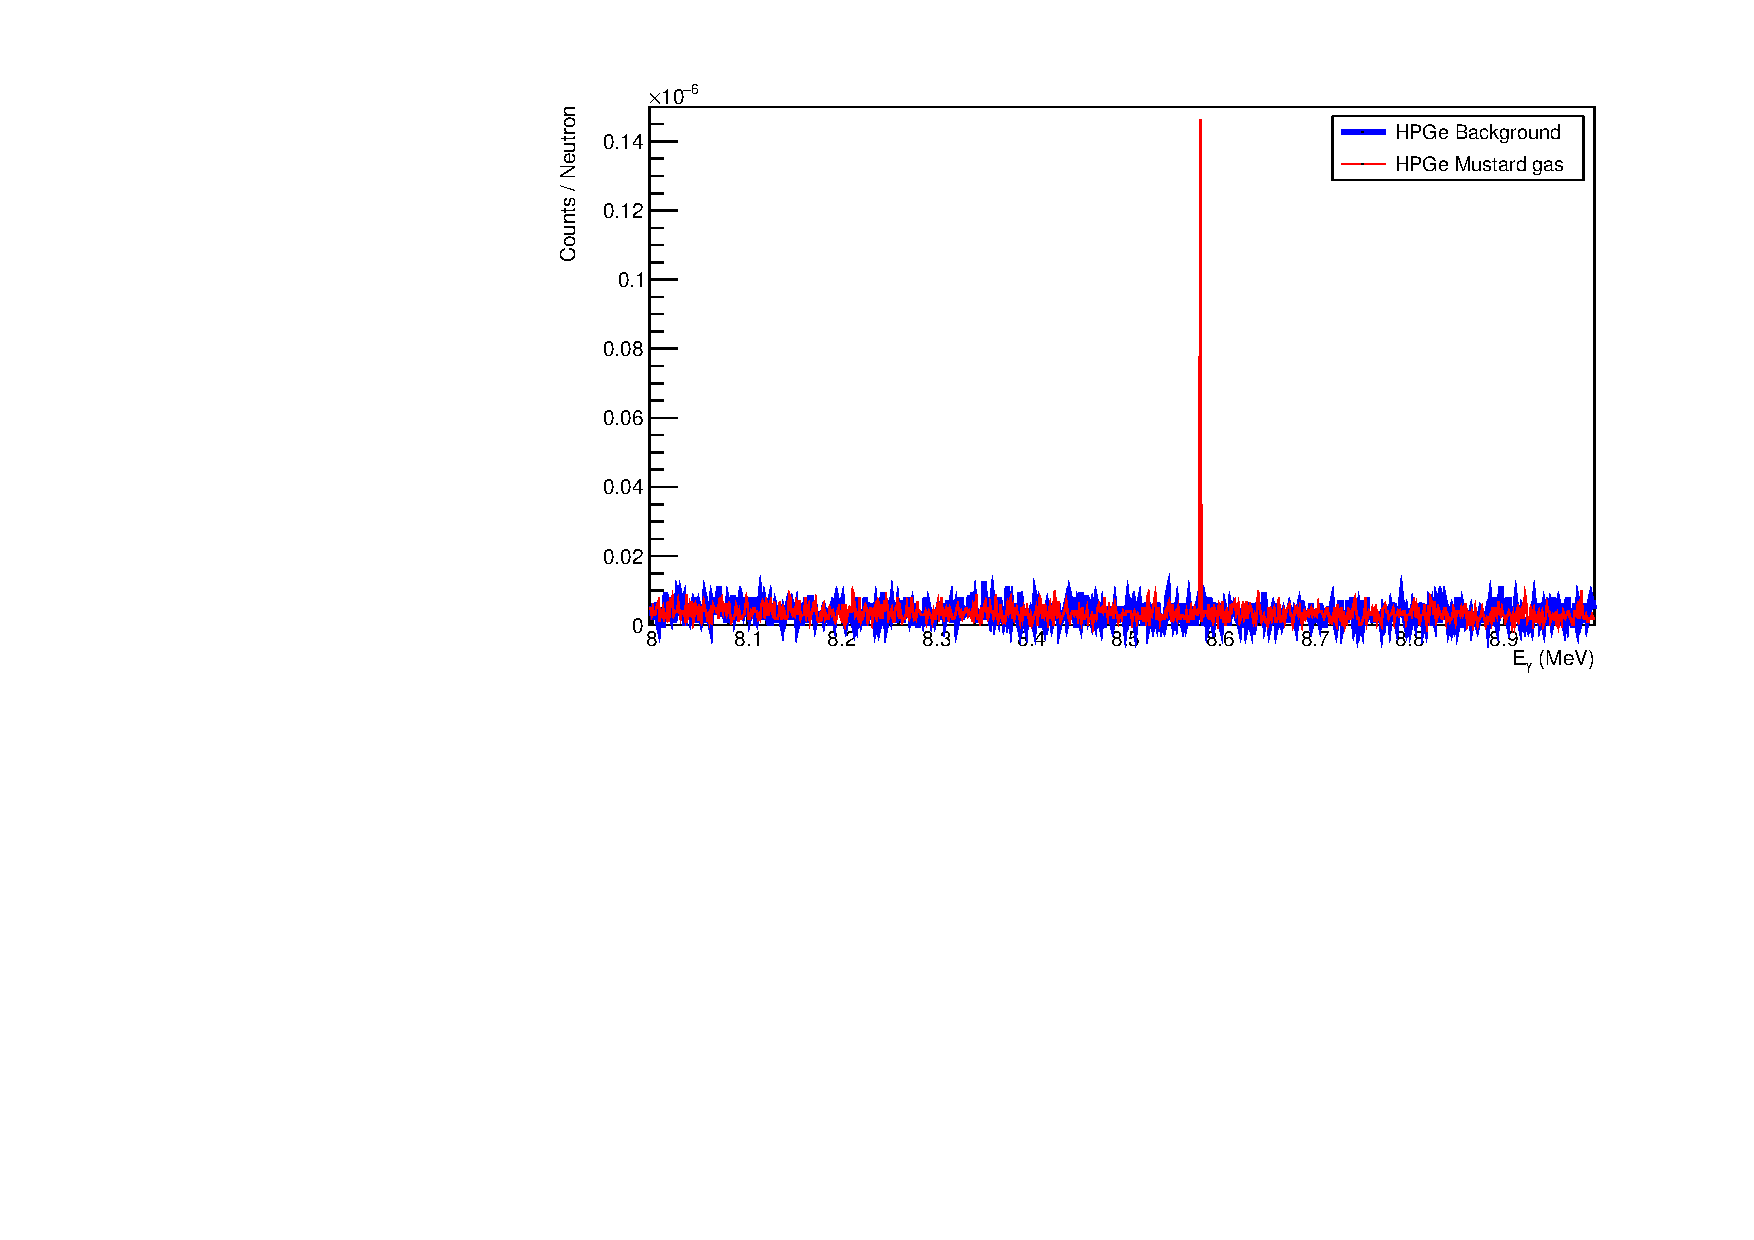
\includegraphics[width=1\textwidth]{res/mustFon89.pdf}
		\caption{Червоним - представлений спектор для Гірчичного газу. Синім - фону} 
		\label{ris:MustFon89}	
	\end{figure} 
	
\newpage

\subsection{Аналіз спектрів $Ag_3AuS_2$}

	За матеріал було обрано ютенбогардтит $Ag_3AuS_2$ - родовища з данними мінералами були знайдені на камчатці поблизу побережжня. Данний мінерал відноситься до рідкисних золотоносних руд, зустрічаеться в природі у твердому стані. Був знайдений на Камчатських родовищах
	
	\begin{figure}[hbt!]
		%\vspace{-10pt}
		\centering 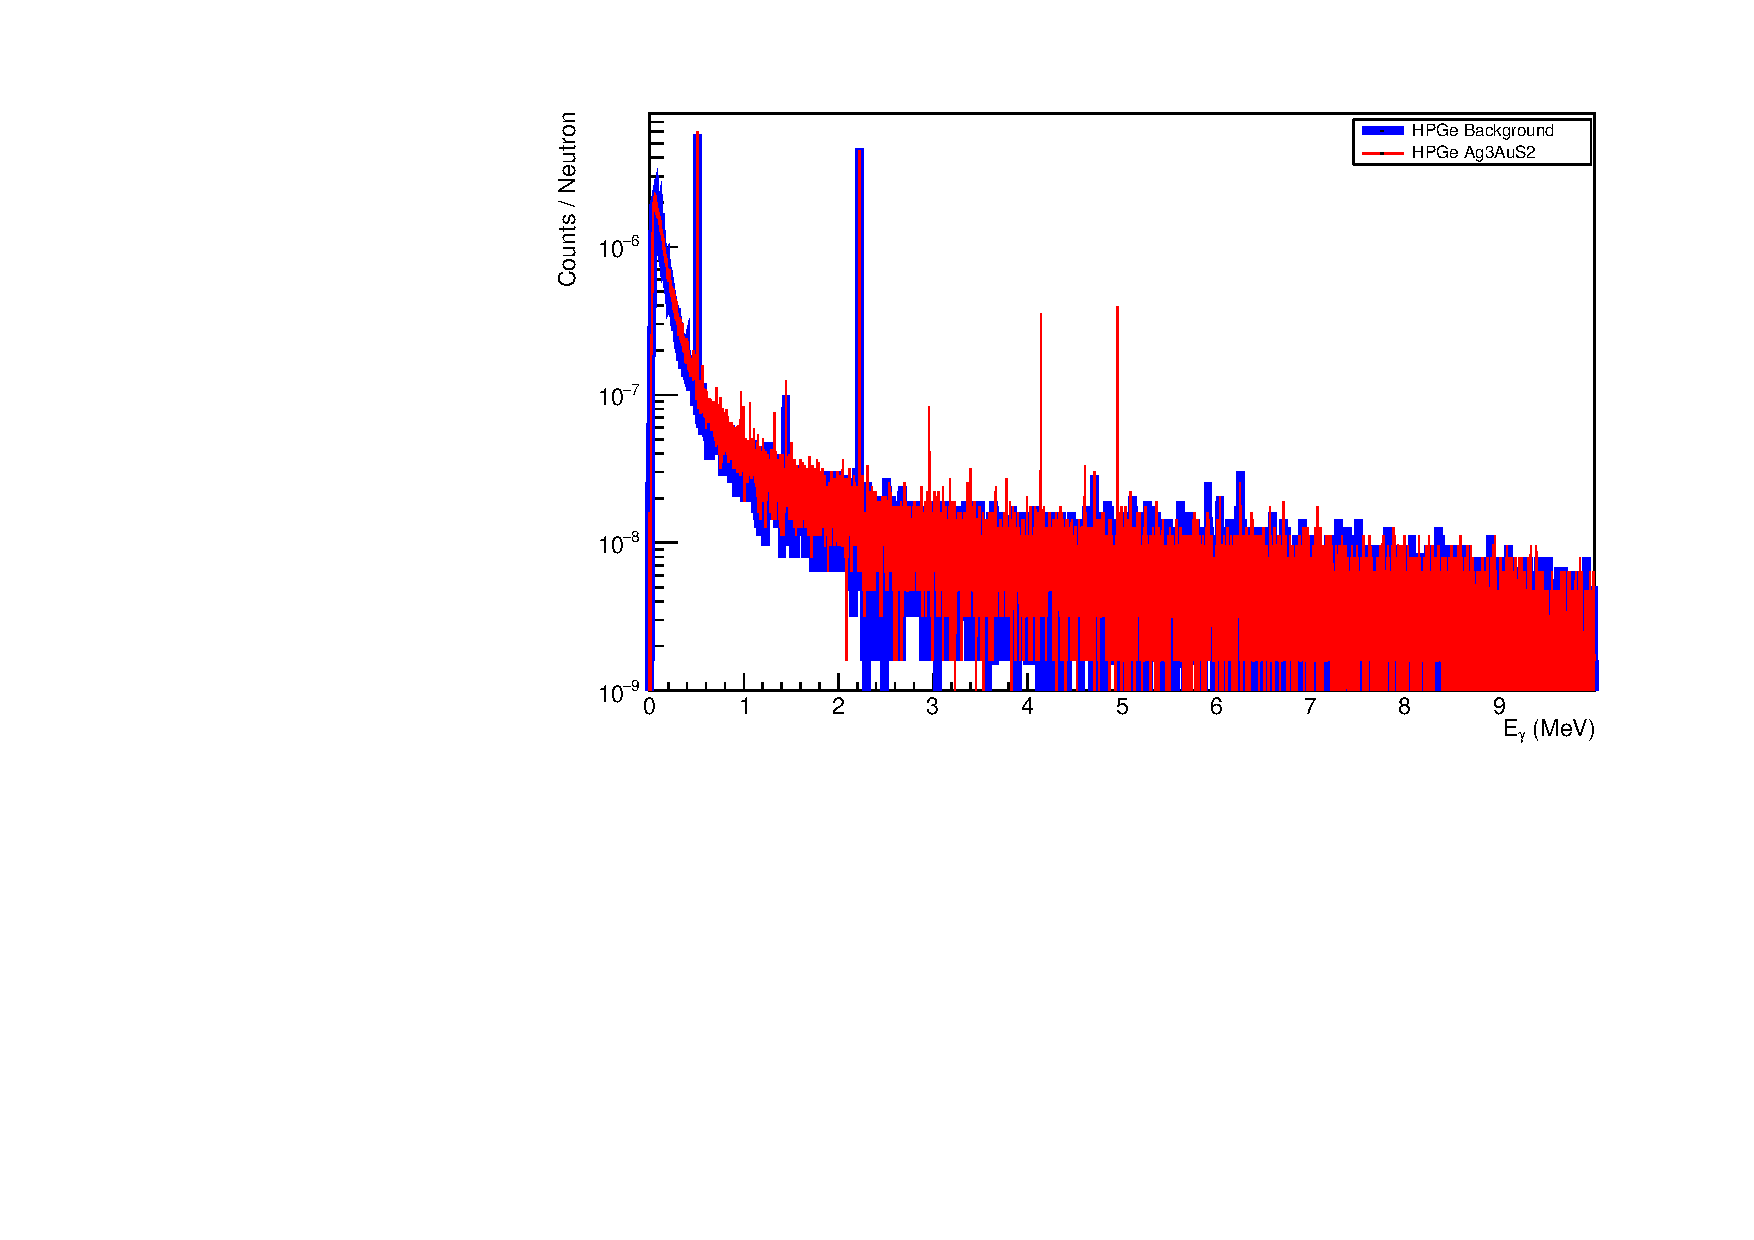
\includegraphics[width=1\textwidth]{res/auFonAllLog.pdf}
		\caption{Червоним - представлений спектор для $Ag_3AuS_2$. Синім - фону} 
		\label{ris:Ag3AuS2Fon}	
	\end{figure} 	

	Данний спектор і фон були набрані при опроміненні нейтронами з джерела максимальної енергією 14.5 МеВ
	Для порівняння було проведенно опромінення за допомгою нейтронів енергією 8.5 та 2.8 МеВ
	\begin{figure}[hbt!]
		%\vspace{-10pt}
		\centering 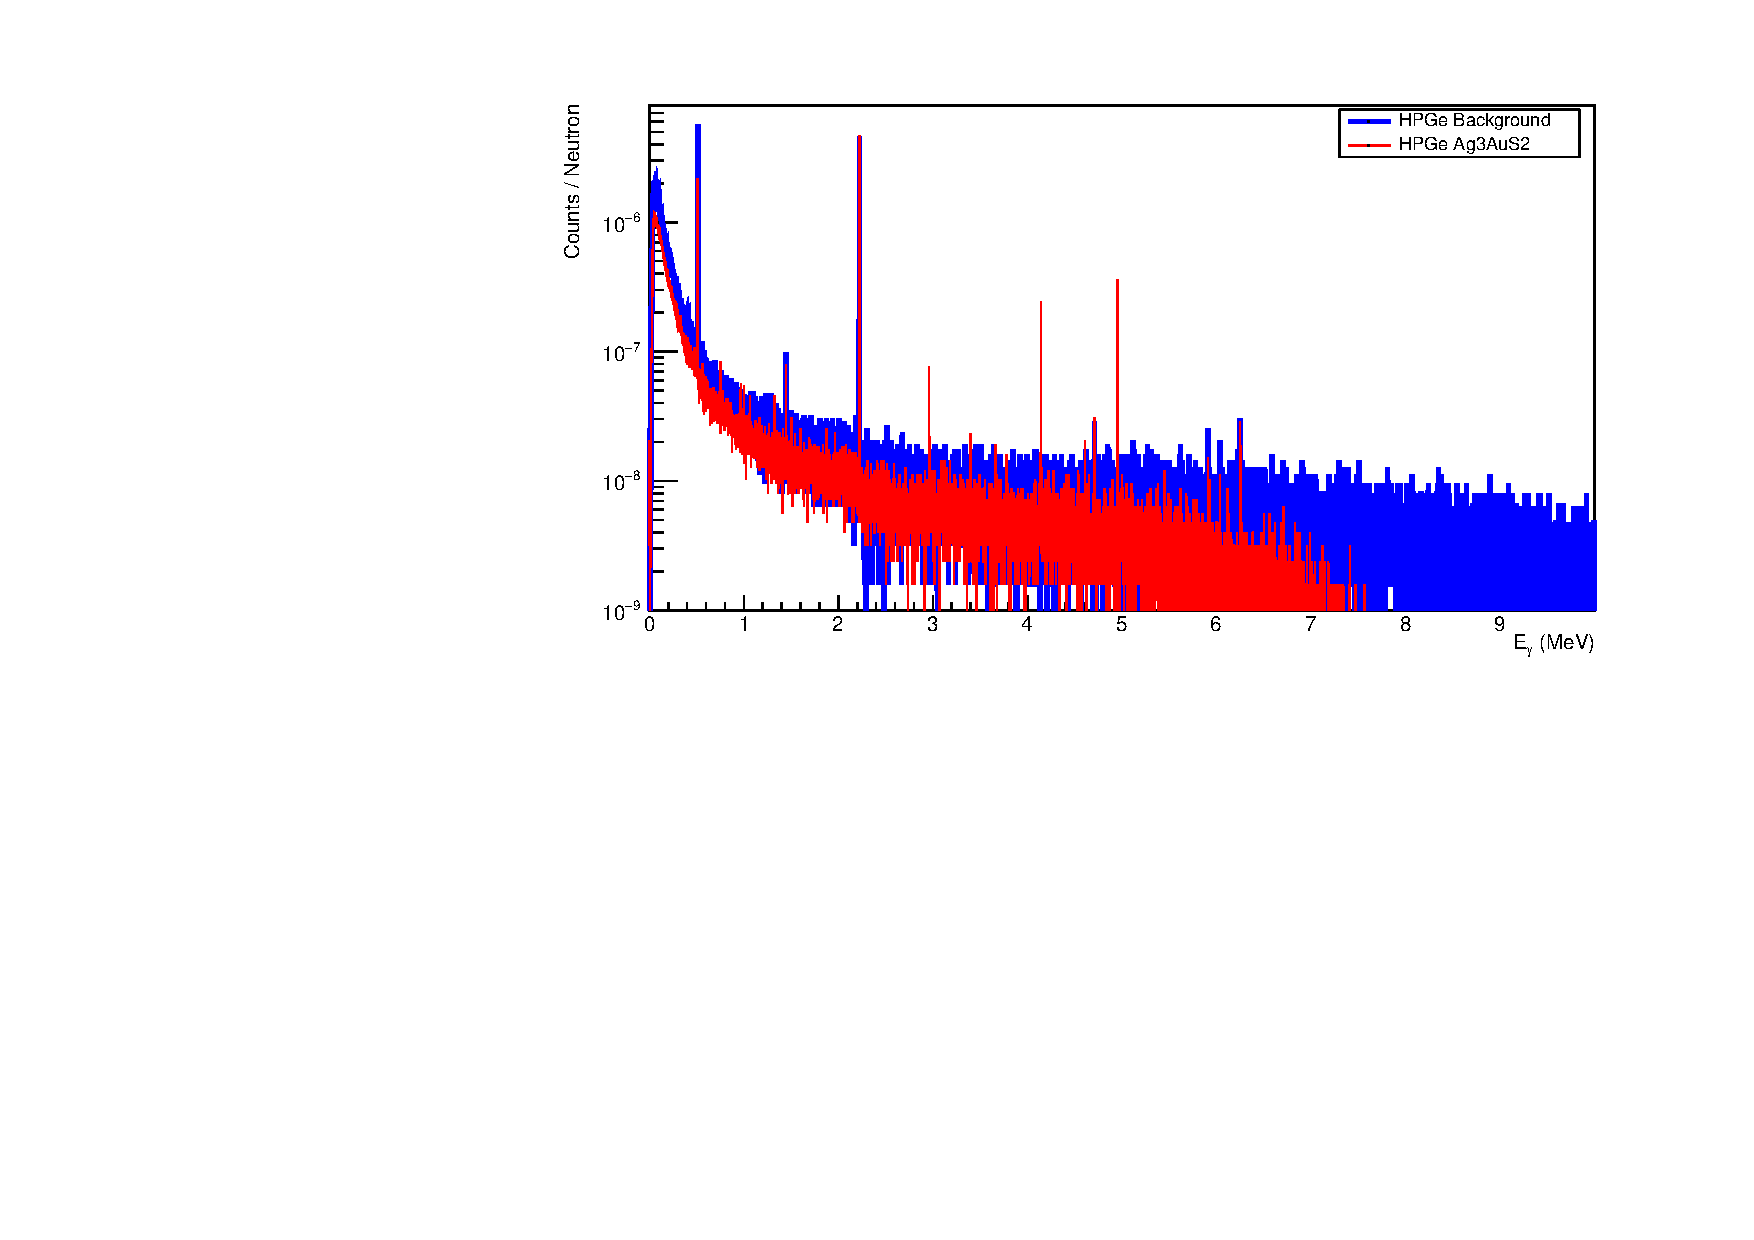
\includegraphics[width=1\textwidth]{res/Ag3AuS2_8_5MeVFonClasic.pdf}
		\caption{Червона - лінія спектру, набраного за опромінення нейтронами 8.5 МеВ}
		\label{ris:Ag3AuS28_5MeV}	
	\end{figure} 
	
	Піки по близу 3, 4 і 5 МеВ майже не втратили інтенсивності тому саме вони були взяті в подальшу обробку. На данному графіку був взятий фон з опромінення 14.5 МеВ нейтронами.
	
	\begin{figure}[hbt!]
		%\vspace{-10pt}
		\centering 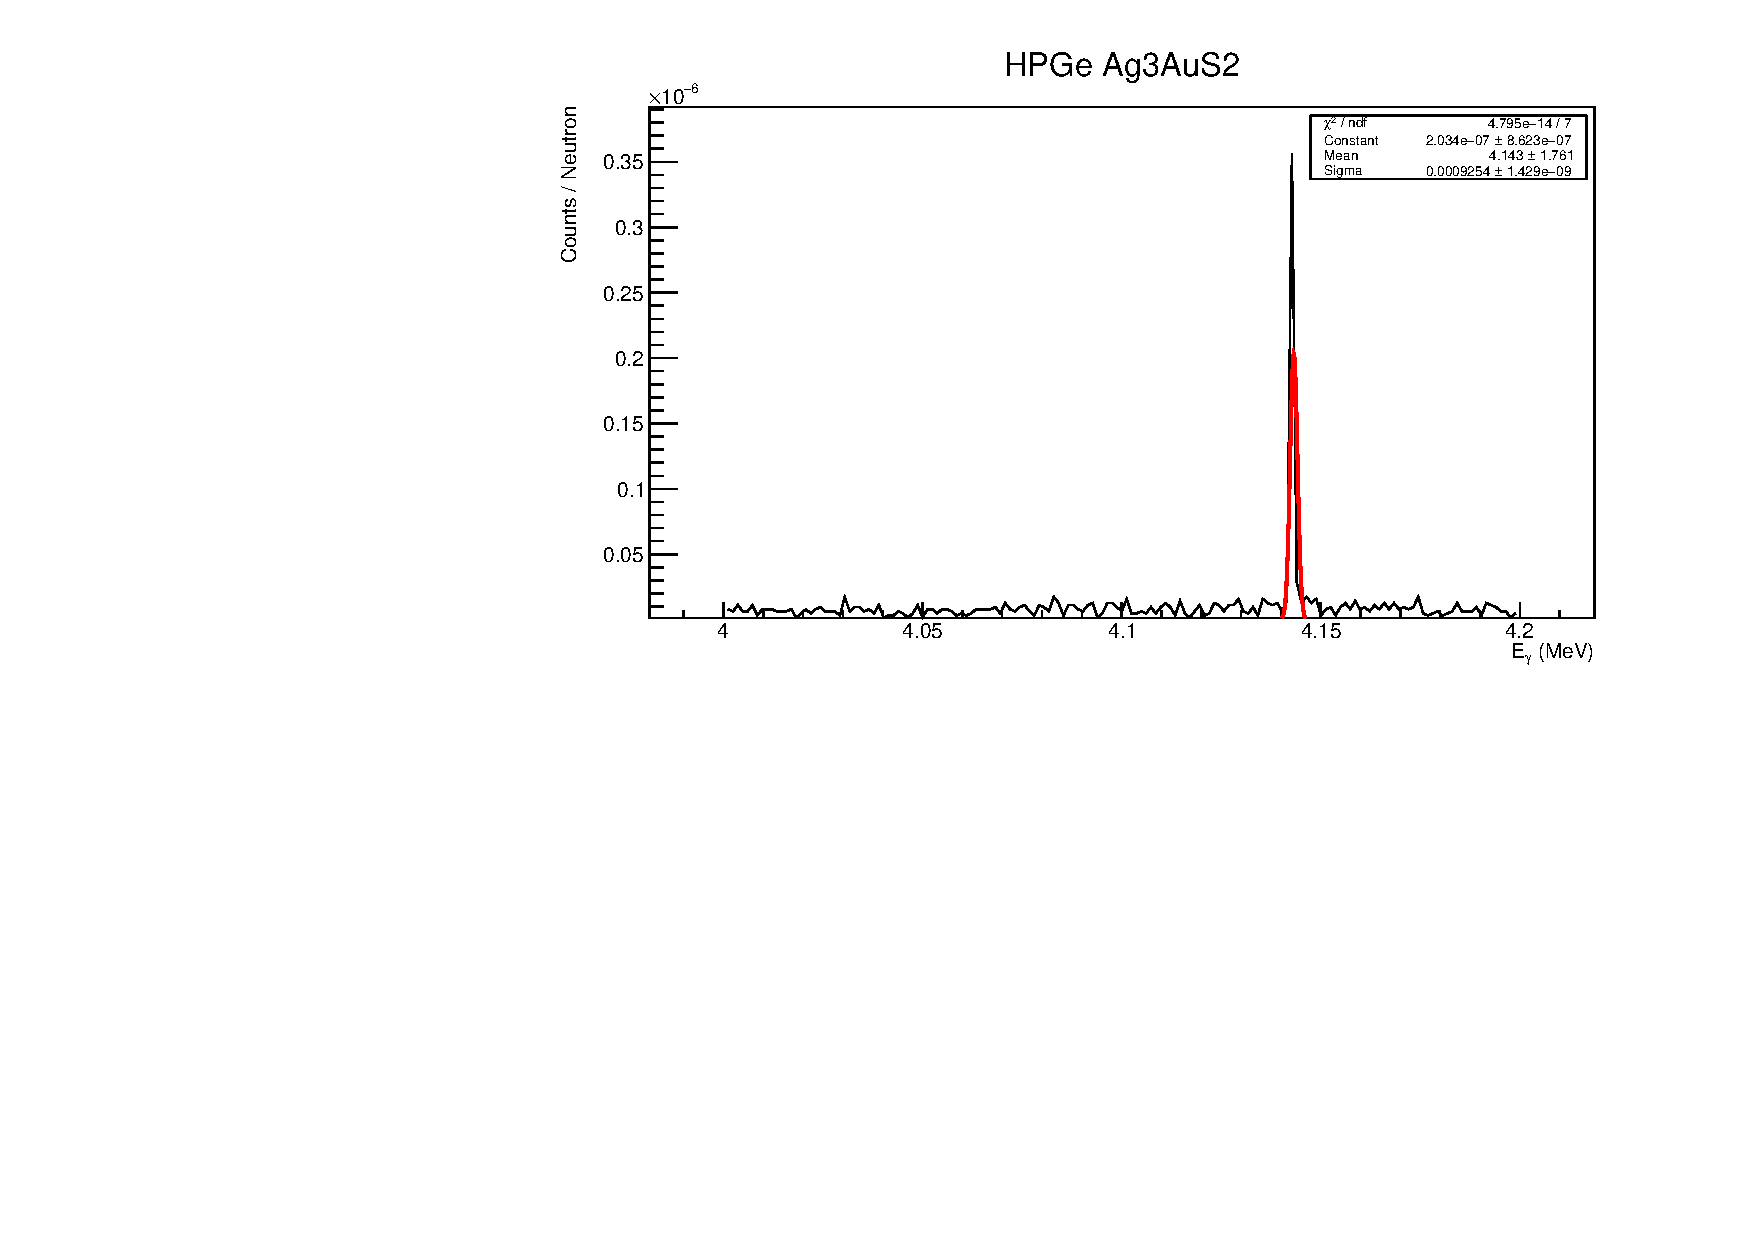
\includegraphics[width=1\textwidth]{res/fit/Ag3AuS24143.pdf}
		\caption{Пік поблизу 4 МеВ}
		\label{ris:Ag3AuS24143}	
	\end{figure} 

\subsection{Аналіз спектрів $CuFeS_2$}
	\begin{figure}[hbt!]
		%\vspace{-10pt}
		\centering 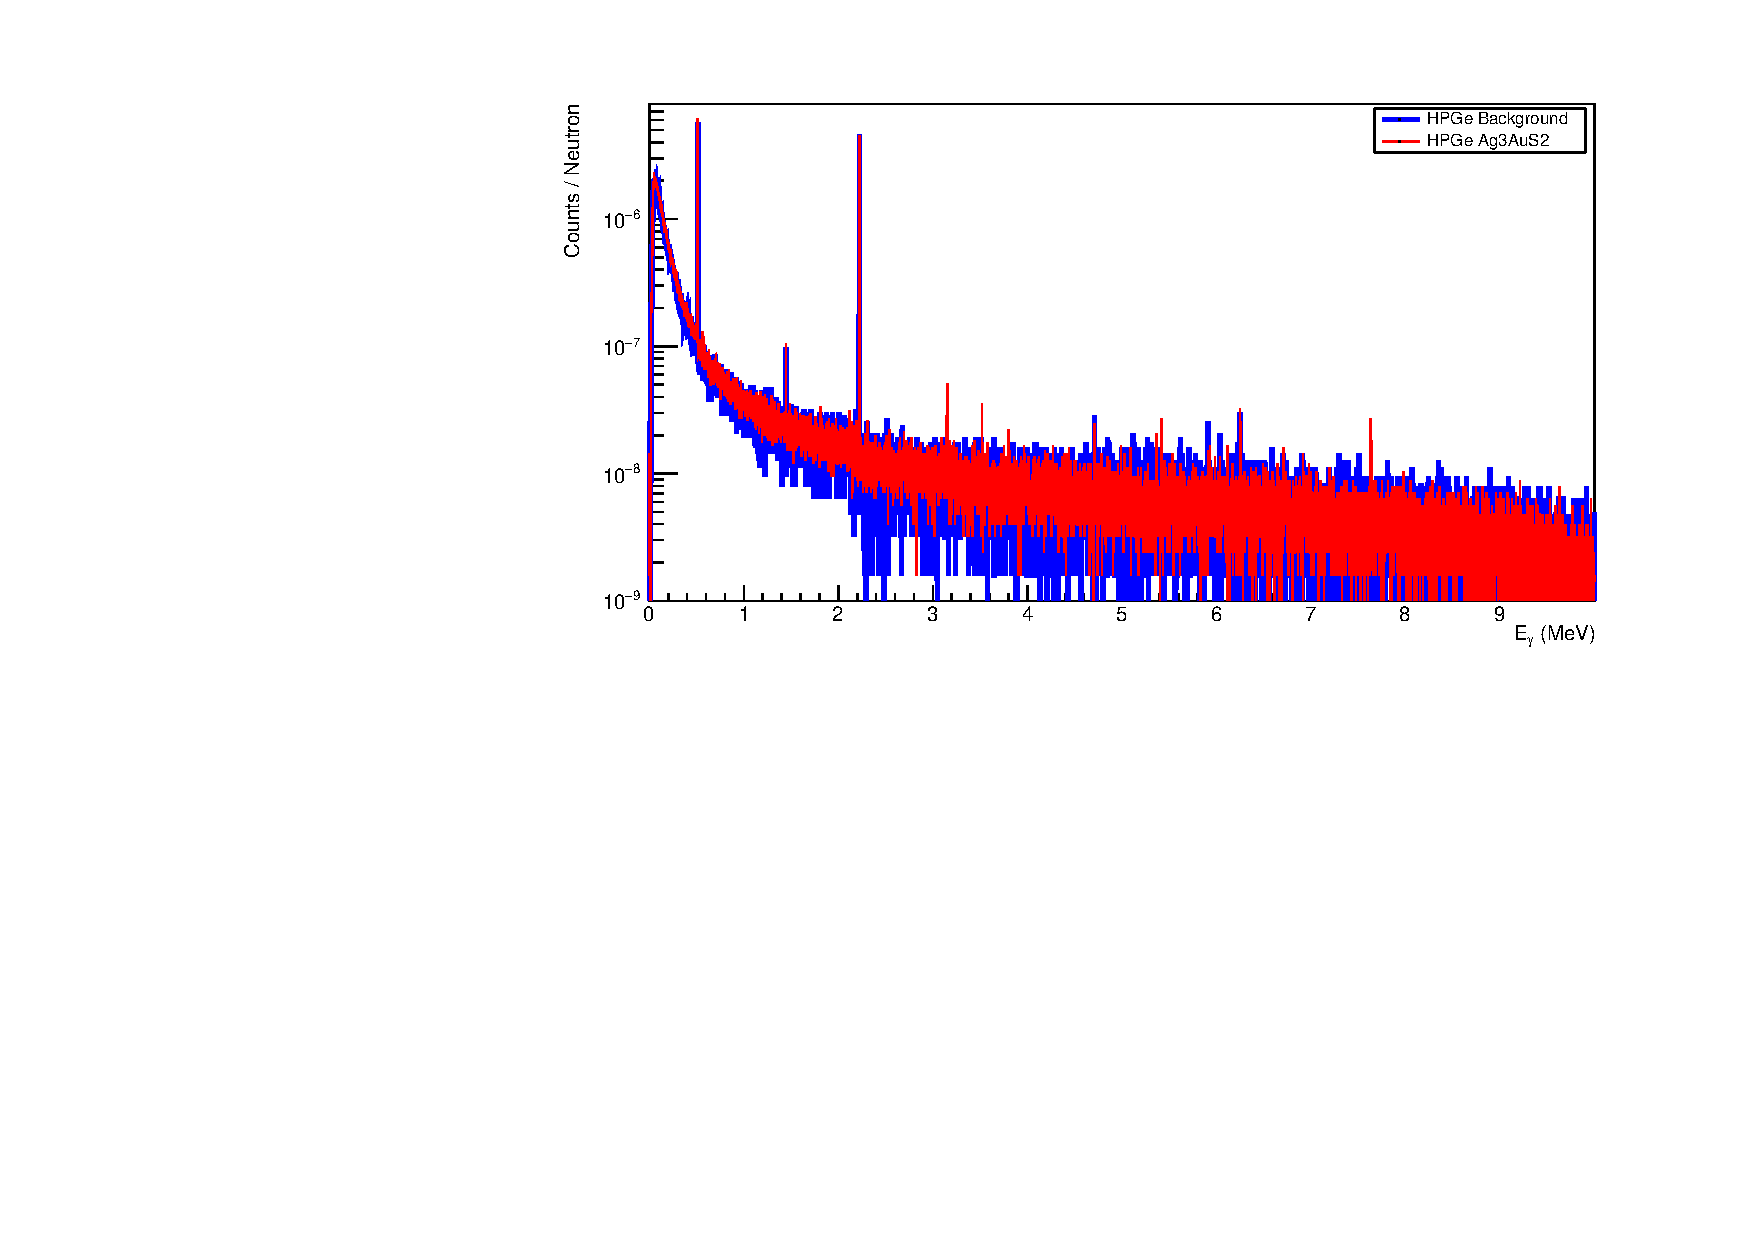
\includegraphics[width=1\textwidth]{res/smCuFeS2FonAll.pdf}
		\caption{Червоним - представлений спектор для $CuFeS_2$. Синім - фону} 
		\label{ris:CuFeS_2Fon}	
	\end{figure} 	
		
\newpage	
%literature
\addcontentsline{toc}{section}{Література}
\begin{thebibliography}{}
	
%	\comment{кометар: це джерело звідки були взяті розміри детектора}  
	\bibitem{1} \textit{R.M. Keyser and T.R. Twomey} - Extended Source Sensitivity and Resolution Comparisons of Several HPGe Detector Types with Low-energy Capabilities \\
	\href{https://www.ortec-online.com/-/media/ametekortec/technical%20papers/high%20purity%20germanium%20detector%20applications%20and%20technology%20developements/extended-source-sensitivity-resolution-comparisons-several-hpge-detector-types-low-energy-capabilities.pdf?la=en}{ HPGe Detector Types}
		
	\bibitem{1} \textit{Aatos Heikkinen, Nikita Stepanov Helsinki Institute of Physics, P.O. Box 64, FIN-00014 University of Helsinki, Finland Johannes Peter Wellisch CERN, Geneva, Switzerland} - Bertini intra-nuclear cascade implementation in Geant4
	\href{https://www.slac.stanford.edu/econf/C0303241/proc/papers/MOMT008.PDF}{link}
	
	\bibitem{1} \textit{Ю.В. Сереткин, Г.А. Пальянова Институт геологии и минералогии им. В.С. Соболева СО РАН} - ИЗОМОРФНОЕ ЗАМЕЩЕНИЕ СЕРЫ СЕЛЕНОМ И МОРФОТРОПНЫЙ ПЕРЕХОД В РЯДУ $Ag_3Au(Se,S)_2$
	\href{https://www.sibran.ru/upload/iblock/478/478309021b63c0dc426e82c4025e6471.pdf}{link}
	
	\bibitem{1} \textit{В. М. Округин1, А. У. Ким} О рудах Асачинского золото-серебряного месторождения
	(Южная Камчатка)
	\href{http://www.kscnet.ru/ivs/publication/volc_day/2014/art51.pdf}{link}
	
\end{thebibliography}

\end{document}
